\documentclass[12pt,a4paper]{article}

\usepackage{amsfonts,amssymb,amsmath,amsthm}
\usepackage{stmaryrd} %for special brackets
\usepackage{lipsum}
\usepackage{graphicx}
\graphicspath{img}
\usepackage[hidelinks]{hyperref}
\usepackage{array}
\usepackage{bm} %for bold in math equations
\usepackage{float} %to force the position of some figures
\usepackage{biblatex}
\usepackage{geometry}
\usepackage{todonotes}
\usepackage{multirow}

\addbibresource{_report.bib}
\geometry{left=2.54cm,right=2.54cm}


\title{Internship Report}
\author{Lucas SALAND}
\date{\today}

\begin{document}
\begin{titlepage}
    \begin{center}
        \Large
        \textbf{Master 1 Data Science}\\
        \vspace*{.5cm}
        \LARGE
        \textbf{Internship report: \\Detection of AI-generated images}\\
        \vspace{1cm}
        \small
        \vfill
        \begin{tabular}{lll}
            Supervisor, & Patrcik Bas & Research Director, CRIStAL, University of Lille\\
            Academic supervisor, & Pierre Chainais & Professor, Centrale Lille, University of Lille\\
        \end{tabular}
        \vspace{1cm}\\
        \large
        Lucas SALAND\\
        University of Lille, France\\
        \today\\
    \end{center}
\end{titlepage}
\newpage
\section*{Acknowledgements}
I would like to express my gratitude to my supervisor, Patrick Bas, for their invaluable guidance, support, and encouragement throughout my internship. Their expertise and feedback played a key role in shaping my understanding and advancing my work during this internship. I am truly grateful for the opportunity to work under their supervision.

\noindent I would also like to extend my sincere thanks to all the members of the team I worked with during the challenge for providing a welcoming and stimulating environment. The collaborative atmosphere was crucial in enabling the completion of this project.

\newpage

\tableofcontents
\newpage

\section*{Introduction}
This M1 internship was carried out at CRIStAL in the SIGMA team under the supervision of Patrick Bas. The internship lasted for three months during which we worked on a challenge from the AID on the detection of images generated by AI.\\
CRIStAL is a laboratory which research focus on computer science, signal and automatic control. It is under the supervision of the University of Lille, CNRS and Centrale Lille. The laboratory is divided in 34 research teams grouped in 9 Thematic Groups. SIGMA team is part of DatInG : Data Intelligence Group. SIGMA is a team of 15 permanent staff which focuses on machine learning, statistics and signal processing. Some of the research topics are Monte-Carlo methods, signal processing with tensorial approaches and information security.
Many events occurs in the lab throughout the weeks. Once a month, a team meeting is done were new members present themselves and the team leader Rémi Bardenet keeps the members of the team updated on various point such as career promotion of members, ongoing projects, problems in the team. Special days are also organized like the SIGMA day where members of SIGMA team make presentation on their current work in the morning and then eat at a restaurant before doing activities in the afternoon. CRIStAL's day is a day during which the director of CRIStAL present the highlights of the year in terms of awards and promotion in the labs as well as explanations on the current partnerships with regional actors. Seminar are held often in the lab with presentations from searcher from outside of the lab. I also assisted to a Phd defense.


The Agence de l'innovation et de défense (AID) launched a challenge on detecting modified or generated images. This challenge aimed at detecting three types of images :
\begin{itemize}
    \item fully AI-generated images;
    \item images partially modified by AI;
    \item images partially modified with more usual image processing tools such as photoshop.
\end{itemize}
This challenge was divided in two tasks : A and B. Task A focused on images fully generated by AI. AId first provided a sample of images to give an idea of what would be the testing data would be. Images provided were compressed with JPEG. Our team identified 3 quality factors for compression: 40, 65 and 90. AID then provided 10000 images on the last day of the challenge. The goal was to identify which images were real and which one were generated. On top of this, we could provide which generator was used to generate images. Task A could be treated as binary classification (task A1) problem with the two classes being real and generated images. It could also be treated as a multi-class classification problem (task A2) where the classes would be the real images and all the generator used. The main difficulty was that the generators used were kept secret until the last day of the challenge.\\
Task B focused on the detection of partially modified images. The objectives were :
\begin{itemize}
    \item detecting real images and modified images;
    \item identifying the tool used for modification;
    \item localisation of modification on images.
\end{itemize}

I worked on the challenge in a team with 3 other interns and 5 permanent staff from SIGMA. During the internship, I worked on task A.


\section{AI-generated images detection}
\subsection{AI image generation}
We should now go over an overview of image generation with AI. In recent years, the quality of images generated with AI models skyrocketed. These models appear as promising new tools for art generation and data augmentation for machine learning. In 2014, Generative Adversarial Networks were introduced by Ian J. Goodfellow and his colleagues in \autocite*{goodfellowGenerativeAdversarialNetworks2014}. A GAN is composed of two main components : a generator and a discriminator. The generator take random vector as input and tries to generate images that are indistinguishable from real images. It tries to fool the discriminator. On the other hand, the discriminator's goal is to differentiate between real data from the training set and fake data produced by the generator.
\begin{figure}[H]
    \centering
    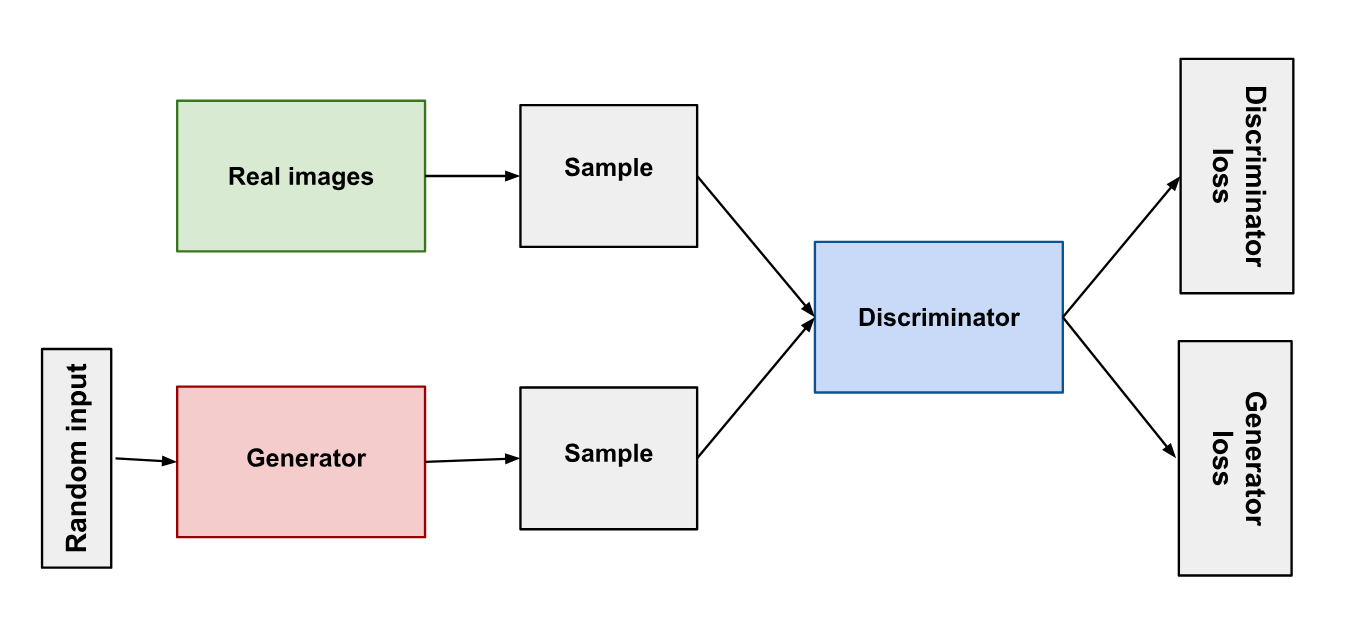
\includegraphics[width=\textwidth]{img/GAN.png}
    \caption{GAN architecture}
\end{figure}

Diffusion models use a different approach to generate images. During training, a diffusion models adds noise progressively to an input image until the image becomes pure noise. It then learns to remove the noise step by step. Once it is trained, it can be used to generate an image from noise. They can also be combined with text prompts to guide the generation process.
\begin{figure}[H]
    \includegraphics*[width=\textwidth]{img/diffusion.png}
    \caption{Image from Wikipedia. Denoising process used by Stable Diffusion.}
\end{figure}

As improvements happen at an impressive rate in the field of generative models, concerns about security issues rose as well. These tools could be used to manipulate information and combined with social media they would be weapon of massive disinformation. As generative model keep improving, we need to develop new tools to detect generated images. But what should we look for in generated images in order to differentiate them from real images? Many approaches were explored in recent years. Let's go over some of them as they are presented in \autocite*{tariangSyntheticImageVerification2024}.

\subsection{Detection based on high-level artifacts}
These methods detect generated images using a similar approach as humans when they differentiate real and generated images. These approaches look at errors such as incorrect perspectives, incoherence in lighting and shadows or asymmetries in faces.

\subsection{Detection based on low-level artifacts}
AI-generated images contain artifacts in the Fourier domain of the model used to generate them. Detecting these traces is a way to detect whether an image is AI-generated. Many generation models contain an upsampling operation in their generation pipeline. An alternative approach to exploit high-frequency artifacts is to look at the noise residuals by removing the scene content. Nonetheless, these approaches are weak to post processing of images. If for instance, jpeg compression is applied, low-level information can be lost making it impossible to correctly classify an image.
\begin{figure}[H]
    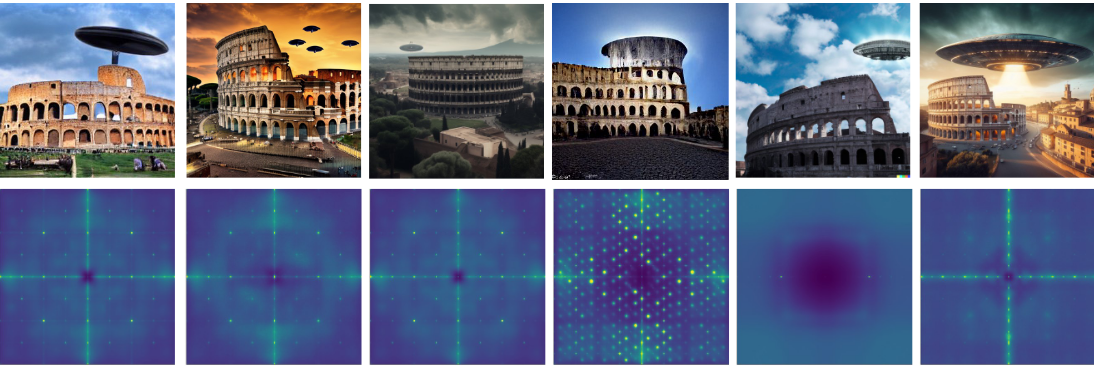
\includegraphics[width=\textwidth]{img/peaks.png}
    \caption{Figure and caption extracted from \autocite*{tariangSyntheticImageVerification2024}. Top: examples of synthetic images, generated using (from left to right) Latent Diffusion, Stable Diffusion, Midjourney v5, DALL·E Mini, DALL·E 2, DALL·E 3. The prompt used for their generation is the following: a photo of the Rome Colosseum with a UFO over it, detailed, 8k. Bottom: Average Power Spectra of the artificial fingerprints for each of such model. Forensic artifacts are clearly visible as spectral peaks in the Fourier domain, stronger or weaker based on the specific model. We can observe that the first three images share very similar artifacts while the fingerprints of the three releases of DALL-E differ greatly from one another, testifying to very different generative architectures.}
\end{figure}

\subsection{Data-driven approaches}
Early method for synthetic image detection were based on CNN architecture with a lot of data. Trying to learn useful features that could help differentiating real and generated images. These first approaches worked well when training and testing data were very similar but had poor generalization capability. To address this robustness issue, researchers used deep CNN architectures combined with augmentation at training time. Augmentations included compressed and blurred images. The diversity of the data used for training also plays a crucial role in a detector's ability to generalize. More recent works delved into architectures different from CNN. In \autocite*{cozzolinoRaisingBarAIgenerated2024}, authors showcased the good performances of CLIP-ViT\footnote{ViT: Vision Transformer} for this type of classification. Within my team, I worked on a semantic approach using CLIP and \autocite*{cozzolinoRaisingBarAIgenerated2024} as a starting point.\\
CLIP (Contrastive Language-Image Pretraining) is a neural networked introduced by OpenAI in \autocite*{radfordLearningTransferableVisual2021}. This network was trained on a massive amount of (text,image) pairs and can then be used with no modification for zero-shot classification. This network training is called contrastive learning. The goal of contrastive learning, as it is stated in \autocite*{tianContrastiveMultiviewCoding2020}, is to learn an embedding that contrasts samples from two distributions. In the case of CLIP, we consider the training dataset to be the following : $\{t_i,\ img_i\}_{i=1}^N$ where $t_i$ is the text associated to the image $img_i$. Each pair contains a textual representation and a visual representation of the same object. We can consider that we thus have a distribution of texts and a distribution of images, which are the marginals, and we have the joint distribution which is the one of the pairs of texts and images. Contrastive learning will separate samles of the joint from sample of the product of marginals. In practice, the model learns to maximize in a latent space the cosine similarity between congruent pairs (e.g.\{"cat", image of a cat\}) and minimize cosine similarity between incongruent pairs (e.g. \{"dog", image of cat\}). As we work in a latent space, it implies that we have encoders to perform the embedding. In the case of CLIP-ViT, transformer-based architectures are used for both the text encoder and the image encoder. Many pretrained versions of CLIP are available online. In our case we used the model proposed by LAION: CLIP ViT-L-14, an open source implementation of CLIP trained on DataComp-1B, a dataset of 1.28B pairs of (text, image) pairs.
\begin{figure}[H]
    \includegraphics*[width=\textwidth]{img/CLIP.png}
    \caption{Figure from \autocite*{radfordLearningTransferableVisual2021}. Images and text are embedded in a latent space, the cosine similarity is then computed on pairs of texts and images.}
\end{figure}

\section{Contributions and associated results}
The first step of building our CLIP detector was to start with something simple. Three ingredients were needed:
\begin{enumerate}
    \item A CLIP model
    \item A dataset with real and generated images
    \item A support vector machine to perform the classification
\end{enumerate}

\subsection{Implementation of a first pipeline toward a CLIP detector}
The CLIP model was obtained through the open-clip library. The weights are loaded from HuggingFace. As a first dataset, we chose ELSA\_D3. This dataset contains 2.31 million quintuples of images. Each quintuples contains one real image and four images generated from a description of the real image with four models of stable diffusion. The dataset being too big for our need and for the available storage space, we only used a small subpart of it. To build our first dataset, we used the datasets library from HuggingFace. We streamed the ELSA\_D3 dataset from HuggingFace and downloaded 10 000 samples from it. At first, we only downloaded pairs of one real image and one generated image from one generator only. Later, we took pairs of one real image and one generated image from a randomly selected generator among the four availables in ELSA\_D3. ELSA\_D3 only contains URLs to the images to download and not the images themselves. Thus, many URLs were dead links. So the code used to download the images had to take into account the possible errors that could occur such as invalid URLs or connection timeout. 

\begin{figure}[H]
    \includegraphics*[width=\textwidth]{img/ELSA.png}
    \caption{An example from ELSA\_D3}
\end{figure}

At first the dataset we created contained the images themselves and every time we wanted to train the SVM\footnote{Support Vector Machine} we had to apply the preprocessing to the images before feeding them to the CLIP model to obtain their embedding. This process being time consuming, we decided to store the features in the datasets instead of the images which lead to significant time savings. The whole process to obtain a classifier was the following :
\begin{itemize}
    \item Load the train/test splits of images
    \item Appply CLIP's preprocessing to all images
    \item Feed the images to CLIP's image encoder
    \item Train an SVM on the CLIP features of the images
    \item Test the SVM
\end{itemize}

\subsection{Impact of JPEG compression}
At first, the SVM was trained on a mix of jpeg and png images. As the sample of images given for the challenge were all jpeg, we decided to convert all images to jpeg. We created datasets for three different quality factors: 40, 65 and 90. These quality factors were chosen based on the early investigations performed on the sample images provided by AID. JPEG compression leads to loss information on the images. Thus we expect that a detector trained on images with high quality factors might perform poorly on  images that are compressed with a low quality factor. 
\begin{figure}[H]
    \includegraphics*[width=\textwidth]{img/jpeg.png}
    \vspace*{-.8cm}
    \caption{Visual impact of JPEG compression}
\end{figure}

To observe the impact of the quality factor on the performances of the detector, we created three datasets, one per quality factor. These datasets are then divided in train and test splits. For each quality factor, we trained the model on the corresponding dataset and tested it ont the 3 test sets. Each dataset contains 10000 elements. We obtain the following results:
\begin{table}[H]
    \centering
    \begin{tabular}{|c|c|c|c|c|}
    \hline
    & \multicolumn{4}{c|}{Test} \\
    \cline{2-5}
     & quality & 40 & 65 & 90 \\
    \hline
    \multirow{3}{*}{Train} & 40 & 0.9813 & 0.9730 & 0.9797 \\
     \cline{2-5}
     & 65 & 0.9450 & 0.9825 & 0.9830 \\
     \cline{2-5}
     & 90 & 0.7744 & 0.8581 & 0.9925 \\
    \hline
    \end{tabular}
    \caption{Accuracy of binary classification for pairs of train/test different quality factors}
    \label{table:jpeg}
\end{table}

As we can obeserve on \autoref*{table:jpeg}, the quality at which images where compressed has an important impact on the average acuracy for binary classification. Looking at the row for quality 40, the accuracy only decrease by a small amount when the testing is perform on images with higher quality factor whereas the acuracy decrease by a significative amount when the data used for training as a high quality factor of 90 and is tested on images with lower quality factor. This result highlight the necessity to add jpeg compression at low quality factor in the training data to obtain better performances.

\subsection{Adding diversity to the data}
We saw in the previous section that our detector as good accuracy when trained on a small quality factor ans tested on other dataset with equal or higher quality factors. But these tests do not give information about the generalization capabilities of our detector. We need to experiment and observe how the SVM classifier performed on images generated by models that are not in the training data. To do so, we used the Synthbuster dataset that was introduced in \autocite{bammeySynthbusterDetectionDiffusion2024}. This datasets contained images generated by 9 different models:
\begin{itemize}
    \item DALL-E 2
    \item DALL-E 3
    \item Adobe Firefly
    \item Midjourney v5
    \item Stable Diffusion 1.3
    \item Stable Diffusion 1.4
    \item Stable Diffusion 2
    \item Stable Diffusion XL
    \item Glide
\end{itemize}

For each generator, 1000 images were generated. This dataset contained only generated images. For testing, we need both real and generated images. Thus we added 9000 images from ELSA\_D3 that were not used in the previous datasets we created.
After training on 10 000 images from ELSA\_D3 with quality factor 40 and testing on synthbuster we obtained an accuracy of 0.64. Our detector was not generalizing well. Two ideas were proposed to improve detector's performances:
\begin{itemize}
    \item Train a multi-class classifier and use it as a binary classifier
    \item Add more diversity in the training data in terms of generators.
\end{itemize}

Implementing the multi-class classifier was simple for the SVM as we just replaced binary labels with class labels and replaced the LinearSVC from sklearn with OneVsOneClassifier. We then trained and tested on Synthbuster and plotted the confusion matrix to see if our classifier could differentiate the images from different generators.

\begin{figure}[H]
    \includegraphics*[width=\textwidth]{img/confusion.png}
    \caption{Confusion matrix for a SVM multiclass-classifier trained and tested on synthbuster.}
\end{figure}

The SVM is able to differentiate pretty well generators on which it has been trained on. It made some mistakes between two versions of stable diffusion but this might be because architectures of both models are similar. This result was a first look at multiclass classification performances but test on out-of-distribution data would be required to see the real performances of our detector.

\subsection{Neural network and bigger datasets}
Up until synthbuster, I was gathering dataset by myself over internet. Then, the team decided to share datasets to be more efficient. Therefore, new datasets were added under a common folder on epeautre, the remote machine on which our code was running and our data was stored. The AID dataset was created. This dataset contained 17 generators with 2000 images per generator and 165000 real images from Flickr. In my case I only took a 1000 images per generators and 17000 real images.\\

Besides the AID dataset we used another dateset that we named AID\_TEST which was used to test the model we trained on AID. This dataset contained 32 generators with 1500 images generated for each of them. In addition to that, the dataset contained 40 000 real images. Training and testing a multiclassifier on datasets thay contains the same classes is simple but what about datasets with classes that do not match? We decided to group generators in families. For instance, all generators that are different versions of Stable Diffusion are grouped together and mapped to the same integer. Instead of predicting the class of specific genertor, our model output the class of a family of generators. To implement thhis, we created three maps:
\begin{itemize}
    \item GEN\_TO\_GEN which maps a string representing a specific generator to its family of generators which is another string,
    \item GEN\_TO\_INT which maps a generator family to an integer
    \item INT\_TO\_GEN which maps an integer to the family of generators
\end{itemize}
\begin{figure}[H]
    \includegraphics*[width=\textwidth]{img/maps.png}
    \caption{The mapping between generators and integers}
\end{figure}

Most generators present in AID\_TEST were variations of those present in AID(except for StyleGAN 2 and 3 that were only present in AID\_TEST). Thus, we decided to add a second dataset for testing: OOD\footnote{Out of distribution. This dataset has been created by Antoine Mariot}. This dataset contained 7 different generators. Most of them were not in AID nor AID\_TEST. A 100 images were generated for each of the following generators: 
\begin{itemize}
    \item Lexica
    \item Ideogram
    \item Leonardo
    \item Copilot
    \item image to image from Stable Diffusion 1.5
    \item photoshop generative magnification
    \item photoshop generative fill
\end{itemize}

As a first experiment on this dataset, we decided to compare accuracy of SVM and neural network for classification. We built a simple 2 layer fully connected network with 16 outputs (15 outputs for generators and one for real images). Since we implemented a neural network with Pytorch, we decided to take the opportunity to replace HuggingFace's datasets library with Pytorch's Dataset class. Indeed, working with HuggingFace's library has proven to be unpractical for our work and slowed down our iterative process since we were creating many variations of datasets. On the other hand, Pytorch's Dataset class was easy to work with and made the code base easier to navigate and understand as the whole code for the datasets was now in a single file. Once our Dataset class for the AID dataset was implemented, we trained our SVM and our neural network on 80\% of the 34000 data points of AID and tested on the remaining 20\%. We tested for both binary (real or generated) and mutli-class (16 classes) classification.

\begin{table}[H]
    \centering
    \begin{tabular}{|c|c|c|}
        \hline
        Model & Binary classification accuracy & Multi-class classification Accuracy\\
        \hline
        SVM & 0.970 & 0.873\\
        \hline
        Neural network & \textbf{0.974} & \textbf{0.878}\\
        \hline
    \end{tabular}
    \caption{Comparison between SVM and neural network for accuracy in classification task.}
    \label{table:svmVsNN}
\end{table}

The neural network has slightly better performances and the developpment of tools is easier with it since we can centralize all the logic in a single class. Hence, we switched from a SVM to a neural network for the classification.\\

Instead of only looking at the accuracy of the model for binary and multi-class classification. We chose to take a look at the accuracy per family of generators to see if some were harder to classify than others. We trained a multi-class classifier model on AID and tested it on binary classification and multi-class classification on the test split of AID (20\% of AID) and on AID\_TEST. We obtained the following results:
\begin{table}[H]
    \centering
        \begin{tabular}{|p{.22\textwidth}|p{.2\textwidth}|p{.15\textwidth}|p{.2\textwidth}|p{.15\textwidth}|}
            \hline
            Generator & Binary Accuracy on Test from AID & Binary Accuracy on AID\_TEST & Multi-class Accuracy on Test from AID & Multi-class Accuracy on AID\_TEST\\
            \hline
            Real & 0.982 & 0.563 & 0.982 & 0.563\\
            \hline
            Stable diffusion & 0.964 & 0.945 & 0.824 & 0.636\\
            \hline
            Kandisky & 0.990 & 0.879 & 0.849 & 0.609\\
            \hline
            DF\_XL & 0.952 & 0.887 & 0.870 & 0.077\\
            \hline
            dreamlike & 0.940 & 0.728 & 0.637 & 0.091\\
            \hline
            gigaGan & 0.861 & 0.810 & 0.740 & 0.281\\
            \hline
            GlideUP & 0.990 & 0.994 & 0.937 & 0.943\\
            \hline
            LafitteUP & 0.995 & 0.998 & 0.991 & 0.995\\
            \hline
            LCM\_Dreamshaper & 0.995 & 0.980 & 0.923 & 0.892\\
            \hline
            megaDallEUP & 0.989 & 0.991 & 0.866 & 0.910\\
            \hline
            miniDallEUP & 0.995 & 0.993 & 0.943 & 0.917\\
            \hline
            pixart & 0.995 & 0.891 & 0.700 & 0.076\\
            \hline
            playground & 0.941 & 0.881 & 0.743 & 0.107\\
            \hline
            styleGan2 & Not in the dataset & 0.748 & Not in the dataset & 0.000\\
            \hline
            styleGan3 & Not in the dataset & 0.682 & Not in the dataset & 0.000\\
            \hline
            animagineXL & 0.989 & 0.988 & 0.904 & 0.423\\
            \hline
        \end{tabular}
        \caption{Accuracy of multi-class classifier on binary classification and multi-class classification}
    \end{table}

The model performed pretty well for binary classification on both AID and AID\_TEST. Nevertheless it struggles to correctly classify real images indicating that it might be biased toward generated images. As for multi-class classification, the model performs well on the test split of AID but the accuracy is significatively lower on AID\_TEST.\\


% issue with our mutliclass approach -> mapping to new generators require training from scratch every time -> weird workflow
We faced somes issues with multi-class classification as we didn't know which generators would be used for the challenge, we couldn't settle on a fixed list of generators when creating dataset. This lead to some inconsistencies when we were introducing new datasets in our workflow. Indeed, each time a dataset was added with generators that could not be matched to any family in GEN\_TO\_GEN, we had to modify the GEN\_TO\_GEN by adding a new family to it. This implies retraining the model since the number of outputs of the model grows everytime a family is added to GEN\_TO\_GEN. To keep things managable and to have an efficient workflow, we decided to focus on binary classification for the CLIP detector. But before dropping the multi-class classifier we compared the accuracy of a binary classfier to the accuracy of a multi-class classifier used for binary classification\footnote{generated images are mapped to "generated" label while real images are mapped to "real" label}. We trained both the binary and multi-class classifier on AID and tested on AID\_TEST. We obtained the following results: an accuracy of 0.71 for the binary model and 0.73 for the multi-class classifier used for binary classification. The difference in accuracy is of 2\% between binary model and multi-class model for binary classification. This difference is big enough to be highlighted but not significative enough to keep working with the multi-class classifier. We thus traded off a little bit of performances for a simpler workflow allowing faster iterations in our developpment process which was needed because of the short amount of time available to develop a solution.\\
While working on the three datasets, we noticed that there was some repetition in the content of the generated images for some generators as we can see on \autoref{fig:repetition}. This repetition in the semantic might not be an issue for residual detectors that looks at low level artifacts. But with CLIP, our goal was to use the content of images as a key information for detection. Having similar generated images in the training data was not desirable. Therefore, we decided to remove the generators that contained many repetitions by creating a generator blacklist for each dataset. AID datset went from 15 generators to 11, 16 generators out of the 32 from AID\_TEST were blacklisted as well. At last, we also removed three generators from OOD: image to image Stable Diffusion 1.5, photoshop generative magnification and photoshop generative fill. OOD didn't contain repetition but the three generators we removed were special case of image generators as they were only partially modifying the images and not fully generating them. The task of the challenge I was working on would not contain images forged with this kind of tools so we decided to remove them from the testing data.

\begin{figure}[H]
    \centering
    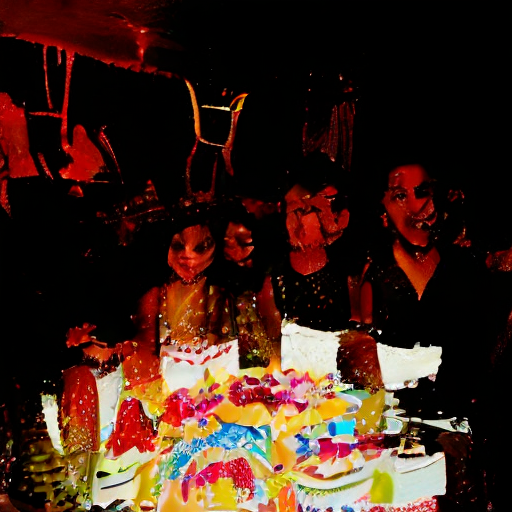
\includegraphics[width=.49\textwidth]{img/birthday1.png}
    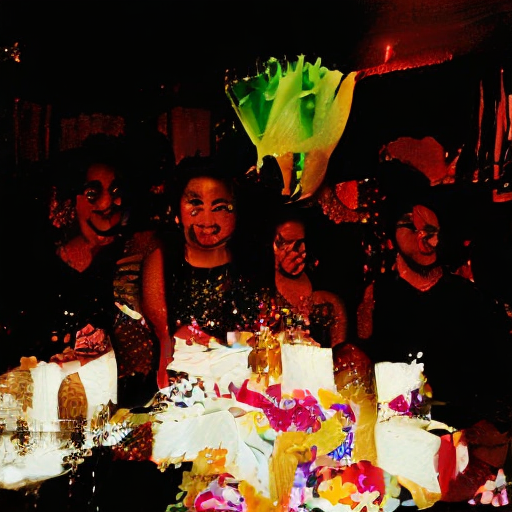
\includegraphics[width=.49\textwidth]{img/birthday2.png}
    \caption{Example of repetition in the content of images. The imgaes are not the same but their semantic is very similar.}
    \label{fig:repetition}
\end{figure}


\subsection{Pair training and fine-tuning}
When we changed from ELSA to AID, AID\_TEST and OOD datasets, we lost a key component of our training: pair training. We designed a new dataset of a 1000 pairs of real and generated images. Images were generated from prompt extracted with an image captioner. Image were generated with only one model: Stable Diffusion. Since we wanted diversity in the training, we kept training on AID and used pair dataset for fine-tuning. A binary model trained on AID without fine-tuning had an accuracy of \textbf{0.82} on OOD. After fine-tuning on the 1000 pairs we obtain an accuracy of \textbf{0.80}. We decided to change our training set. Instead of training on AID and then fine tuning on the 1000 pairs we created a single dataset: FlickrAndPairs. This datasets contained the 1000 pairs of real and generated images as well as 1000 images from Flickr and 1000 generated images from AID. The binary classifier was trained from scratch on this dataset and we obtained an accuracy of \textbf{0.83} on OOD. The increase in performance was not significative enough to conclude that FlickrAndPairs dataset was better for training. We built a dataset meta\_test thay was designed to have a wide range of generators. Many of it's data came from the already existing AID\_TEST set and images of generators that were not in AID\_TEST were generated manually. We thus trained a model on FlickrAndPairs and fine-tuned it on meta\_test. We kept a split of meta\_test for testing to see the improvement in performances before and after fine-tuning. The fine-tuning helped improve accuracy across all generators as it was expected. We then tested on OOD to see if this fine-tuning lead to improvement in accuracy. The accuracy greatly improved on OOD after fine-tuning on test\_meta as we can see on \autoref{tab:fine-tuning}. But this is mainly due to the fact that test\_meta contains generators that are present in OOD.

\begin{table}[H]
\centering
    \begin{tabular}{|c|c|c|}
        \hline
        Generator & Before fine-tuning & After fine-tuning\\
        \hline
        Real & 0.937 & 0.977 \\
        \hline
        animagineXL3 & 0.800 & 1.000 \\
        \hline
        SDXL & 0.508 & 0.938 \\
        \hline
        gigaGan & 0.346 & 0.889 \\
        \hline
        Copilot & 0.961 & 1.000 \\
        \hline
        Dreamshaper & 0.922 & 0.969 \\
        \hline
        kandinsky & 0.784 & 1.000 \\
        \hline
        LongCaptions & 0.807 & 0.943 \\
        \hline
        SD1\_5 & 0.365 & 0.921 \\
        \hline
        Lexica & 0.915 & 0.974 \\
        \hline
        dreamlike & 0.638 & 0.983 \\
        \hline
        MidJourneyV6 & 0.895 & 0.974 \\
        \hline
        Leonardo & 0.728 & 0.880 \\
        \hline
        SD2\_1 & 0.489 & 0.957 \\
        \hline
        stylegan2\_3 & 0.121 & 0.989 \\
        \hline
        pixartAlpha & 0.831 & 0.986 \\
        \hline
        playground & 0.859 & 0.953 \\
        \hline
        pixartSigma & 0.781 & 1.000 \\
        \hline
        DF-XL & 0.136 & 0.951 \\
        \hline
        Ideogram & 0.805 & 0.974 \\
        \hline
    \end{tabular}
    \caption{Accuracy comparison on test\_meta's test split before and after fine-tuning on test\_meta.}
\end{table}

\begin{table}[H]
    \centering
    \begin{tabular}{|c|c|}
        \hline
        accuracy on OOD before fine-tuning on meta test & 0.83 \\
        \hline
        accuracy on OOD after fine-tuning on meta test & 0.91 \\
        \hline
        accuracy on test meta before fine-tuning on test meta & 0.79 \\
        \hline
        accuracy on test meta after fine-tuning on test meta & 0.97 \\
        \hline
    \end{tabular}
    \caption{Accuracy comparison before and after fine-tuning.}
    \label{tab:fine-tuning}
\end{table}

\subsection{Integration with other detectors to build a meta-classifier}
Our team developped several detectors in parallel that were then merged into a meta classifier. Each detector produces softmax for an image and these softmax are then concatenated into a single vector. This vector of softmax is then used as input for the meta classifier. On the day of the challenge, we received the 10 000 images and extracted the softmax of every images with each detectors and fed the softmax to the meta classifier. We wanted to have an idea of the accuracy of our model so we decided to manually label the 10 000 images. Me, Antoine Mariot and Amandine Roure labelled 3333 images each. The CLIP detector achieved 0.89 accuracy on task A\footnote{Detection of purely generated images}. We saw the main ideas we developped in order to complete the challenge from AID. We will now go over some additional approach that we explored but were not used for the final submission either because the idea lacked substantial results or because it was done after the deadline for the submission.

\subsection{Color features}
When looking at the colors of real and generated images, we are often able to tell which image is real based on the saturation of the colors and the palette used. From this observation we think that color features might be an interesting features to include with the CLIP features. We looked at the histograms of real images and generated images in RGB, HSV (Hue, Saturation, Value), YCbCr spaces to see if we noticed some differences. We then wanted to inlcude them with CLIP features. After discussing the idea, we came to the conclusion that information about colors might already be present on CLIP features. On top of that, the preprocessing applied to both real and generated images modify the colors  of the images as we can see on \autoref*{fig:preprocessing}, making this information less relevant to distinguish real and generated images.

\begin{figure}[H]
    \centering
    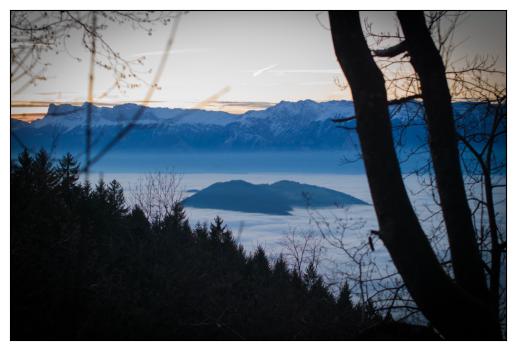
\includegraphics[height=.3\textwidth]{img/img.png}
    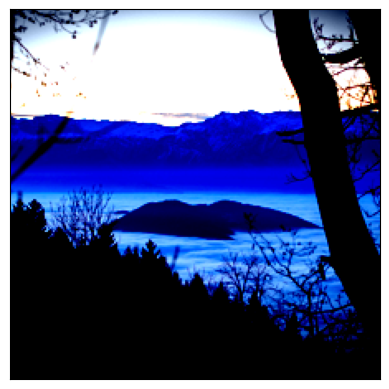
\includegraphics[height=.3\textwidth]{img/img_preprocess.png}
    \caption{Image before and after CLIP's preprocessing.}
    \label{fig:preprocessing}
\end{figure}

\subsection{DoubleCLIP: another approach to work with pairs}
The idea we had with DoubleCLIP is to upgrade the pair training with more features. For each image, we extract a long caption with BLIP, a pretrained model that can be used for Image-Text retrieval. We then use this caption as a prompt to generate an image using Stable Diffusion XL 1.0. Our hope was that for fake images, their CLIP features would be similar to the CLIP features of the images generated with the prompt extracted and real images would have CLIP features that would be more different from their images generated with the extracted prompt. 
\begin{figure}[H]
    \centering
    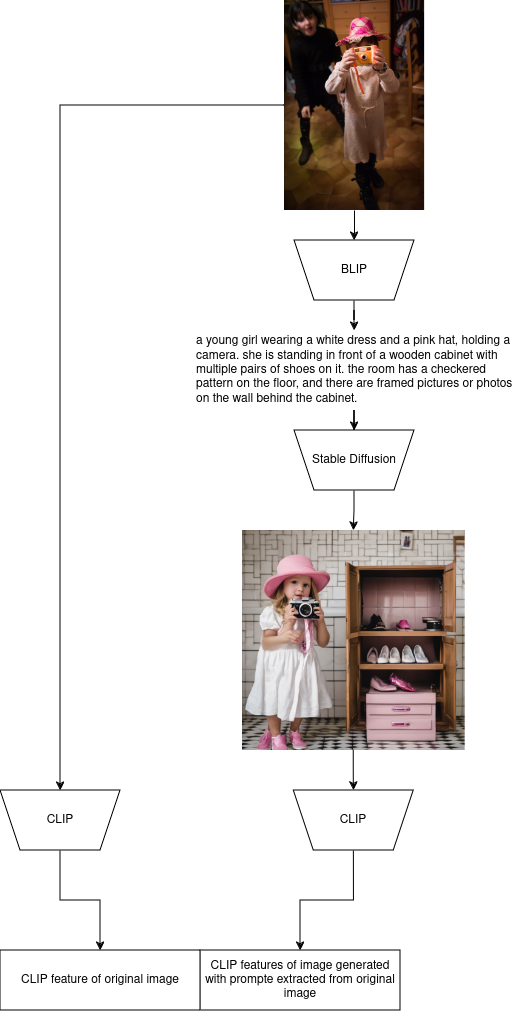
\includegraphics[width=.45\textwidth]{img/double_clip.png}
    \caption{The pipeline to create double clip features.}
\end{figure}
We trained a model on 400 images and tested on 1600 images from the dataset of real and generated pairs. Retrospectively, doing so was a mistake as there is no need to have more testing images than training images. We obtained an accuracy of 0.98 for DoubleCLIP against 0.99 for CLIP. Unfortunately, we cannot appreciate a real difference in performances between using DoubleCLIP features and CLIP features since we were already at a high accuracy on this dataset. Using an other dataset for testing would have been better to appreciate the difference in performances. Since the generation part of the pipeline to extract doubleCLIP features was computationaly expensive and took a lot of time, we decided to focus on other ideas.

\subsection{DINO as an alternative to CLIP}
CLIP is the model we chose to embed images into a latent space. Nevertheless, we could have picked an other model to extract features. We experimented with DINOv2, a pretrained model for visual feature extraction that was introduced in \autocite*{oquabDINOv2LearningRobust2024} by Meta AI Research and Inria. We trained two models: a model that was learning from CLIP features and one that would learn from DINOv2 features. We trained both of them on FLickrAndPairs and tested them on the manually labeled data from Task A. We did so in order to compare to the accuracy of the model we used for submission in the challenge. The model using CLIP features obtained an accuracy of \textbf{0.86} while the model trained on DINOv2 features got an accuracy of \textbf{0.76}. The model used for the submission of the challenge had an accuracy of \textbf{0.88} but it is worth noting that the model used for the challenge was trained on FlickrAndPairs and then fine-tuned on test\_meta. The DINOv2 features did not seem to outperform CLIP's features. We decided to train a model that would learn from the concatenation of CLIP and DINOv2 features. We obtained an accuracy of  \textbf{0.89} which was not a significant improvement compared to the \textbf{0.88} of the model used for the challenge.

\subsection{Tip-Adapter}
Most of the effort was put into trying to build datasets to improve performances of our detectors. We wanted to explore other methods to build a classificator. Instead of changing the data, we wanted to change the detection pipeline. The approach taht we discussed previously in this report, extracting CLIP features and fedding them to a neural network, is called linear probing. In \autocite*{khanCLIPpingDeceptionAdapting2024}, the authors compared four methods for real/fake classification with CLIP features:
\begin{itemize}
    \item linear probing
    \item fine-tuning
    \item prompt tuning
    \item CLIP adapter
\end{itemize}
Linear probing does not fully take advantage of CLIP. Indeed, it only uses the image encoder and completly drops the text encoder. Prompt tuning uses both the image and text encoders. The classification is performed by looking at the cosine similarity between the visual features and the text features of a prompt that is the concatenation of a learned prompt with "real" or "fake" (see \autoref*{fig:classification}).
Fine-tuning is an option, but it is computationaly expensive as it requires updating the weights of both encoders. The final method proposed was CLIP adapter. CLIP is a pretrained model that can extract visual features that can be used for zero-shot classification. The idea of CLIP adapter is to provided features that are more suited to the problem of real/fake classification. A neural network takes as input CLIP's visual features and generate new features from them. Adapted features and original features are then added together in order to retain information from the pretraining. The classification is then performed with the cosine similarity between the features and the embedding of "real" and "fake" texts. 

\begin{figure}[H]
    \includegraphics*[width=\textwidth]{img/classification.png}
    \caption{Figure from \autocite*{khanCLIPpingDeceptionAdapting2024} presenting four different approaches to perform real/fake classification with CLIP.}
    \label{fig:classification}
\end{figure}

While reading the paper for CLIP adapter, we discovered that a new version of CLIP adapter was introduced in \autocite*{zhangTipAdapterTrainingfreeAdaption2022}: Tip-Adapter. A method designed for few-shot classification using CLIP.

\begin{figure}[H]
    \includegraphics*[width=\textwidth]{img/tip_adapter.png}
    \caption{Figure and caption from \autocite*{khanCLIPpingDeceptionAdapting2024}. The Pipeline of Tip-Adapter. Given a K-shot N-class training set, we construct a cache model to adapt CLIP on downstream tasks. It contains few-shot visual features $F^T_{train}$ encoded by CLIP and their ground-truth labels $L^T_{train}$ under one-hot encodings. After retrieval from the cache model, the few-shot knowledge is incorporated with CLIP’s pre-trained knowledge, achieving the training-free adaption. In our case N=2 and C=768.}
    \label{fig:tip}
\end{figure}

\newcommand\ft{$F_{train}$}
\newcommand\lt{$L_{train}$}

Let's review how Tip-adapter works. Tip-adapter is built upon the combination of two type of knowledge: CLIP's knowledge and few-shot knowledge. CLIP's knowledge is obtained by computing the cosine similarity between CLIP visual features for a given image and CLIP textual features for "real" or "generated". If we use this knowledge alone, we would perform what is called zero-shot classification with CLIP. Tip-Adapter adds additional data which is called few-shot knowledge. We build a cache of real and fake images. This cache contains two matrices: \ft\ and \lt\ (see \autoref*{fig:tip}). \ft\ is a matrix of dimension (N*K)$\times$C where N is the number of classes (2 in our case), K is the number of images per class and C is the dimension of the space in which images are embedded with CLIP's image encoder. Each row represents the CLIP encoding of a given image in the training data. The K first row are the \textbf{normalized} CLIP features for the K fake images and the K remaining rows are the \textbf{normalized} CLIP features of the real images. \lt\ is a (2*K)$\times$ 2 matrix representing a one-hot encoding of the labels. In our implementation, [1,0] represents a fake image while [0, 1] represents a real image. We will explain the role of this matrix later. The goal is to obtain logits and to look at the index of the maximum logit to classify an image as real or fake. The logits are obtained with the following formula:

\begin{equation}
    logits = \alpha\underbrace{\varphi(f_{test}F_{train}^T)L_{train}}_{\text{Few-shot knowledge}} + \underbrace{f_{test}W_c^T}_{\text{prior knowledge of pretrained CLIP}} \nonumber
\end{equation}

\newcommand{\irow}[1]{% inline row vector
  \begin{smallmatrix}(#1)\end{smallmatrix}%
}
Let's analyse this formula:
\begin{itemize}
    \item $f_{test}$: L2 normalized CLIP features of the input image,
    \item $F_{train}$: matrix of L2 normalized CLIP features of train images,
    \item $f_{test}F_{train}^T$: vector of cosine similarities between CLIP features of the test image and CLIP features of train images,
    \item $\varphi$: $\varphi(x) = \exp(-\beta(1-x))$, turns cosine similarities into non negative values,
    \item $\alpha$ is the weight of the few shot-knowledge. It is used to balance few-shot knowledge with CLIP's prior knowledge. If the classification we want to perform is close to the pretraining of CLIP, then lower values of alpha are wanted and if the classification task is very different from CLIP's pretraining then higher values of $\alpha$ are desired.
    \item $\varphi(f_{test}F_{train}^T)L_{train}$: vector that contains sum of cosine similarities with respect to each class. $L_{train}$ is used as a convenient way to obtain these sums. For our binary classification problem, we obtain the following equation:
    \begin{equation}
        \varphi(f_{test}F_{train}^T)L_{train} = \Bigl({\displaystyle\sum_{k=1}^K{f_{test} F_{train}[k]^T}},
        \ \displaystyle\sum_{k=K+1}^{2K}{f_{test} F_{train}[k]^T} \Bigr)\nonumber
    \end{equation}
    \item $W_c^T$: text embedding of our classes. For our binary classification it contains the text embedding of "a generated image" and "a real image".
    \item $f_{test}W_c^T$: logits obtained with CLIP prior knowledge
\end{itemize}

For our experiments, the data used in the cache of Tip-adapter was from FlickrAndPairs and we tested it on two of our datasets: test\_meta and taskA. We obtained the following results:
\begin{table}[H]
    \centering
    \begin{tabular}{|c|c|c|}
    \hline
    \textbf{Cache Size} & \textbf{Accuracy on TaskA} & \textbf{Accuracy on test\_meta} \\ \hline
    2    & 0.68 & 0.65 \\ \hline
    4    & 0.69 & 0.71 \\ \hline
    6    & 0.70 & 0.74 \\ \hline
    8    & 0.75 & 0.74 \\ \hline
    16   & 0.72 & 0.77 \\ \hline
    32   & 0.69 & 0.75 \\ \hline
    64   & 0.60 & 0.71 \\ \hline
    128  & 0.70 & 0.76 \\ \hline
    200  & 0.68 & 0.76 \\ \hline
    1000 & 0.69 & 0.75 \\ \hline
    2000 & 0.68 & 0.75 \\ \hline
    \end{tabular}
    \caption{Accuracy on TaskA and test\_meta of Tip-adapter for different cache sizes with $\alpha$=5. The accuracy doesn't improve much once 3 (cache size 6) or 4 (cache size 8) images per class are provided.}
    \label{tab:cache}
\end{table}

\begin{table}[H]
    \centering
    \begin{tabular}{|c|c|c|}
    \hline
    \textbf{Alpha} & \textbf{Accuracy on TaskA} & \textbf{Accuracy on test\_meta} \\ \hline
    0 & 0.65 & 0.47 \\ \hline
    1 & 0.74 & 0.65 \\ \hline
    2 & 0.75 & 0.71 \\ \hline
    3 & 0.76 & 0.73 \\ \hline
    4 & 0.75 & 0.74 \\ \hline
    5 & 0.75 & 0.74 \\ \hline
    \end{tabular}
    \caption{Accuracy on TaskA and test\_meta for different values of alpha with a cache size N*K=100. When $\alpha$=0, this is the same as using CLIP for zero-shot classification. When we use few-shot knwoledge, we improve the accuracy. This shows the importance of using this knowledge to obtain a better accuracy.}
    \label{tab:alpha}
\end{table}

Now that the inner working of Tip-Adapter is clearer, we can move on to an improved version of it: Tip-Adapter-F. Tip-Adapter-F is Tip-Adapter with fine-tuning. As explained in \autocite*{zhangTipAdapterTrainingfreeAdaption2022} the values in \lt\ are seen as good initialization for learnable parameters that are fine-tuned through SGD. For our experiment, we fixed a cache size of 100 and used the same data from FlickrAndPairs as we used for Tip-Adapter. Besides, $\alpha$ was set to 5.

\begin{table}[H]
    \centering
    \begin{tabular}{|c|c|}
    \hline
    \textbf{Number of epochs} & \textbf{Accuracy on taskA} \\ \hline
    5   & 0.85 \\ \hline
    10  & 0.86 \\ \hline
    20  & 0.88 \\ \hline
    50  & 0.89 \\ \hline
    100 & 0.90 \\ \hline
    \end{tabular}
    \caption{Tip-Adapter-F Accuracy on TaskA for different number of epochs for fine-tuning. We denote a significative improvement of Tip-adapter-F over Tip-adapter.}
\end{table}

\section{Conclusion and perspectives}
During this internship, I had the opportunity to work on a problem through different perspectives. The main focus has been on the data as we tried to find how we should gather data and what kind of images we wanted to train our detector on. We saw that pair training was not enough to get good performances. We saw that we could also try a similar approach just by swapping CLIP with DINOv2 but this did not result in improved accuracy. We also explored tip-adapter to use CLIP features differently from our initial approach and we saw improvement with Tip-Adapter-F. We also had some surprises with the challenge from AID. We thought that real images would have an important semantic content but the real images provided by AID were crops with very poor content. We consider that the data from AID was not the best one. Indeed, if the goal is to leanr how to differentiate real images from generated ones, what is the purpose of providing real images that do not conrespond to the one that would be analysed in practice? Even though the real images we trained on were pretty different from the ones provided for the challenge, we still obtained a 0.88 accuracy. Our initial intuition was that CLIP extracted semantic content and we wanted ti use this to build an efficient detector. Nonetheless, our detector still obtained good accuracy on real images with poor semantic content.  To improve this work, we would need to understand what CLIP features represent. To do so we could perform adversarial attack with projected gradient descent to see what kind of signal would make our detector switch from one class to the other.\\
This internship was an opportunity for me to improve my technical skills with because I learned how to use PyTorch and to work remotely through ssh and keeping track of my work with git. I also iproved my ability to work in autonomy on complex subjects through article reading. It has been a great learning opportunity.

\newpage
\printbibliography

\end{document}